%%%%%%%%%%%%%%%%%%%%%%%%%%%%%%%%%%%%%%%%%
%
% CMPT 435
% Assignment Four
%
%%%%%%%%%%%%%%%%%%%%%%%%%%%%%%%%%%%%%%%%%

\documentclass[letterpaper, 10pt]{article} 

\usepackage[english]{babel} % English language/hyphenation
\usepackage{graphicx}
\usepackage[lined,linesnumbered,commentsnumbered]{algorithm2e}
\usepackage{listings}
\usepackage{xcolor}
\usepackage{float}
\usepackage{fancyhdr} % Custom headers and footers
\pagestyle{fancyplain} % Makes all pages in the document conform to the custom headers and footers
\usepackage{lastpage}
\usepackage{url}
\usepackage{multirow}

\definecolor{codegreen}{rgb}{0,0.6,0}
\definecolor{codegray}{rgb}{0.5,0.5,0.5}
\definecolor{codepurple}{rgb}{0.58,0,0.82}
\definecolor{backcolour}{rgb}{0.95,0.95,0.92}

\lstset{       
    language=c++,
    backgroundcolor=\color{backcolour},   
    commentstyle=\color{codegreen},
    keywordstyle=\color{magenta},
    numberstyle=\tiny\color{codegray},
    stringstyle=\color{codepurple},
    basicstyle=\ttfamily\footnotesize,
    breakatwhitespace=false,         
    breaklines=true,                 
    captionpos=b,                    
    keepspaces=true,                 
    numbers=left,                    
    numbersep=5pt,                  
    showspaces=false,                
    showstringspaces=false,
    showtabs=false,                  
    tabsize=2                    
}

\fancyhead{} % No page header
\fancyfoot[L]{} % Empty left footer
\fancyfoot[C]{page \thepage\ of \pageref{LastPage}} % Page numbering for center footer
\fancyfoot[R]{}

\renewcommand{\headrulewidth}{0pt} % Remove header underlines
\renewcommand{\footrulewidth}{0pt} % Remove footer underlines
\setlength{\headheight}{0pt} % Customize the height of the header

%----------------------------------------------------------------------------------------
%	TITLE SECTION
%----------------------------------------------------------------------------------------

\newcommand{\horrule}[1]{\rule{\linewidth}{#1}} % Create horizontal rule command with 1 argument of height

\title{	
   \normalfont \normalsize 
   \textsc{CMPT 435 - Fall 2024 - Dr. Labouseur} \\[10pt] % Header stuff.
   \horrule{0.5pt} \\[0.25cm] 	% Top horizontal rule
   \huge Assignment Four -- Dynamic Programming and Greedy Algorithms \\     	    % Assignment title
   \horrule{0.5pt} \\[-0.25cm] 	% Bottom horizontal rule
}

\author{Tyler DeLorey \\ \normalsize tyler.delorey1@marist.edu}

\date{\normalsize\ December 6th, 2024}

\begin{document}
 
\maketitle % Print the title

%----------------------------------------------------------------------------------------
%   CONTENT SECTION
%----------------------------------------------------------------------------------------

% Reset figure numbering to include section number
\renewcommand{\thefigure}{\thesection.\arabic{figure}}

\tableofcontents

\section{Introduction}
\subsection{Reused Files}

\noindent
Before I explain what I did for this assignment, I want to explain some files that I've implemented in this assignment that were used in previous ones. The two files that I used were the Stack class (from Assignment 1, used for my implementation of Dynamic Programming in this assignment) and the Sort file (from Assignment 1, reused in Assignment 2, and used for my implementation of the Greedy Algorithm in this assignment). 

\vspace{1em}

\noindent
Like with Assignment 1, the Stack class and its functions are all declared and initialized in my Stack.h file, and it has three functions associated with it: push, pop, and isEmpty. However, unlike the first assignment, I'm using the Vertex object (explained in Section 2) instead of Nodes to push and pop on the Stack. 

\begin{figure}[H]
  \centering
  \lstinputlisting[firstline=1, firstnumber=1, lastline=35]{Stack.h} 
  \label{fig:figure1.1-part1}
\end{figure}

\begin{figure}[H]
  \centering
  \lstinputlisting[firstline=36, firstnumber=36]{Stack.h} 
  \caption{The Stack Class (Stack.h)}
  \label{fig:figure1.1-part2}
\end{figure}

\noindent
The Stack I implemented is essentially a linked list of Vertices with a pointer named "top" that points to the Vertex on top of the Stack. Each Vertex has a member named "next", which points to another Vertex, and it is used by the Stack class to create this linked list. The three functions associated with this class have the time complexity of $O(1)$, meaning they run in constant time. 
\noindent
\begin{itemize}
  \item The "push" function puts some Vertex on top of the Stack. The top pointer of the Stack will be updated to be the Vertex that was passed into the function. The previous top of the Stack (if there was any) will now be the second Vertex on the Stack (Lines 15-20).
  \item The "pop" function removes the top Vertex from the Stack and returns it if it isn't empty. It also sets the new top to the Vertex referenced by the previous top's next pointer (Lines 23-34).
  \item The "isEmpty" function checks whether the Stack is empty by seeing if the top pointer references a valid Vertex (Lines 37-40).
\end{itemize} 

\noindent
Part of my Greedy Algorithm implementation requires some vector to be sorted in descending order. The sort that I use for the vector is Quick Sort because it has a time complexity of $O(n * log(n))$, which is faster than Selection Sort and Insertion Sort, which have time complexities of $O(n^2)$. I chose Quick Sort over Merge Sort is because Quick Sort is an in-place sort, meaning the algorithm doesn't need any more than a constant extra amount of space to perform. I'm not going to show images of the Sort.h file because there wasn't anything that was changed for the most part. The only things that were changed was the data type of the vector used, which uses the Spice object (which will be explained in Section 3) instead of a string (for the previously implemented magicItems), and also it sorts the objects in the vector in descending order (which just required changing data types and the comparison values were changed to the Spice's unit price, which will all be explained in Section 3). The Sort.h is also a lot longer than the Stack.h file, so I don't find it necessary to show this file that was barely changed.

\vspace{5em}

\subsection{Text Files}
\noindent
This assignment has a couple of text files that are used as input for the program to run. The code that I implemented to read this file and to implement its command will be explained in the upcoming sections, but for now, I just wanted to explain the content of these files. The two files that are used are called graphs2.txt and spice.txt. The graphs2.txt file is used for the Dynamic Programming section, and the spice.txt file is used for the Greedy Algorithms section.

\vspace{1em}
\noindent
Below is a snippet of the graphs2.txt file (don't mind the highlighted syntax, doesn't apply for .txt files):
\begin{figure}[H]
  \centering
  \lstinputlisting[lastline=23]{graphs2.txt} 
  \caption{First Directed Graph in File (graphs2.txt)}
  \label{fig:figure1.2}
\end{figure}

\noindent
The file is very similar to the graphs1.txt file used for Assignment 3. Like previously, there are commands, and there are commands like "new" (Line 1) and "add" (Lines 3-7 for vertices, Lines 8-17 for edges) that need to be read and interpreted in certain ways. However, there is now weight to each edge in the graph, and even though it doesn't explicitly say it, it is also a directed graph, meaning each edge has a certain direction that goes from one Vertex to another. There are many aspects about the Vertices and the weights that I can explain now, but I think its best to save all of that information when explaining Dynamic Programming and Single-Source Shortest Path (SSSP). I just want to show the layout of the file so the file reading parser I created is understandable given the commands.

\vspace{1em}
\noindent
Below is the entire spice.txt file used for the Greedy Algorithm implementation. The file is shorter, so why not show it all. Also, there are many differences with this file when comparing it with files from other assignments.

\begin{figure}[H]
  \centering
  \lstinputlisting[]{spice.txt} 
  \caption{Spice Text File (spice.txt)}
  \label{fig:figure1.3}
\end{figure}

\noindent
The first portion of this file contains each Spice object that needs to be created (Lines 4-7). This will be explained in-depth later, but each Spice has a name, a total price, and a quantity. With these Spices in place, the greedy algorithm will run for each knapsack, which have different capacities (Lines 10-14). Basically, as will be explained, for this fractional knapsack problem, the algorithm will try to maximize the value (price per unit) of the spices, which are loaded into the knapsack. It tries to solve the problem of "How do you fill your knapsack to achieve a maximum value?" The implementation I used to answer this question will be explained in Section 3, so stay tuned!

\section{Dynamic Programming}
\setcounter{figure}{0} % Reset figure counter

\subsection{File Parser and Keywords}
\noindent
The first part of this assignment I will explain for this program is the Dynamic Programming implementations. To do this, the program first creates a directed weighted graph, and then using that graph, a Single-Source Shortest Path (SSSP) algorithm is ran to see the shortest path between the first Vertex in the Graph and all other Vertices. Before I explain the parsing I created for the graphs2.txt file, I want to explain some variables I created to help with the process. On the next page, there are declarations of some variables that are used for the parser:

\begin{figure}[H]
  \centering
  \lstinputlisting[firstline=18, firstnumber=18, lastline=32]{main.cpp} 
  \caption{Variable Declarations (main.cpp)}
  \label{fig:figure2.1}
\end{figure}

\vspace{1em}

\noindent
\begin{itemize}
    \item The "file" ifstream variable will store all of the information for the file. In this case, it will store the graphs2.txt file, but it will later be used by the Greedy Algorithm portion of this Assignment (Line 19)
    \item The "line" string will eventually store each line of the file when the parser read it (Line 20).
    \item The "myGraph" pointer points to the current Graph instance that is being worked with (Line 27). The Graph class will be explained later, but it has many similarities to the undirected Graph class that was created in the previous Assignment 
    \item The "check" boolean will decide whether or not to process the current Graph (Line 28). This variable is only set the false in the beginning, and once the first Graph is created and initialized, the boolean will be set to true, and it will remain true for the rest of the program's duration.
    \item The "graphNum" integer stores what Graph the program is currently on (Lines 29). This is only used for output.
    \item The "Index" integers are used to avoid putting magic numbers all over my program (Line 32). This will be explained in-depth later, but each line of the file is put into a vector. These values are used to access certain indices of the vector. For example, the initial word for the command is stored in index 0, the type of command is in index 1, so commandIndex is 0 and typeIndex is 1. This will make more sense when dealing with the parser.    
\end{itemize}

\noindent
I had to read the file and understand all the keywords that were being used in order to create a parser and do tokenization based on each line in the file. Below is how I created a parser for the Graph file.

\begin{figure}[H]
  \centering
\lstinputlisting[firstline=34, firstnumber=34, lastline=78]{main.cpp} 
  \label{fig:figure2.2-part1}
\end{figure}

\begin{figure}[H]
  \centering
  \lstinputlisting[firstline=79, firstnumber=79, lastline=98]{main.cpp} 
  \caption{File Parsing for Directed Graph (main.cpp)}
  \label{fig:figure2.2-part2}
\end{figure}

\noindent
I took a slightly different approach parsing this file compared to parsing the undirected Graph file in the previous assignment. Instead of reading only the necessary words from each line as I processed it, I first read all the words on a line and stored them in a vector. Then, I accessed the vector to process the data. I found this method to be significantly more readable.

\vspace{1em}
\noindent
The first thing I needed to do was to read the file and store it in the file variable (Lines 35-40). After reading the entire file, I needed to process each line of the file (Line 43). There are a couple more local variables to help with the parsing process, which are:
\begin{itemize}
    \item The stream variable is used to convert a single line of text into individual words (Line 45). It can be used to extract each word sequentially using the $>>$ operator.
    \item The word variable, which is a string that takes the value of the stream variable and uses it throughout the if statements in the parser (Line 46).
    \item The words vector is used to store each word of the line, as explained earlier (Line 47). 
\end{itemize}

\noindent
The first section of the parser after the variable declarations is filling up the words vector with each word in the line. Each word in the line is read using the stream and word variables (Line 50). Depending on the word, the program will do the following:
\begin{itemize}
    \item If the word was a comment or was just empty, then no vector needs to be created and the loop is finished (Lines 53-56).
    \item If the word wasn't a comment, that means it is valuable information the program needs to know. Therefore, no matter what, the word will be added to the vector. However, there is one slight problem. Some of these words have semicolons at the back, which is no good when I have to deal with those values. If the word ends in a semicolon, it will be removed (Lines 59-62). Then, the word will be added to the words vector (Line 65).
\end{itemize}

\noindent
As is evident, the file needs to be written in a certain way so the parser can work as intended. If the file format is different in any way, the parser won't function as intended, and it would probably not work in general.

\vspace{1em}
\noindent
After each word in the line was written into the words vector, I needed to find out the possible options for each command. The two words that the commands can start with are "new" or "add", and I would have to ignore anything else. After checking if the vector actually had words in it (Line 68), I would need to check each word in order to fulfill its purpose.

\begin{itemize}
    \item If the word at the first index (Index 0) in the vector was "new", and the word in the second index (Index 1) was "graph", that means that a new Graph would need be created (Line 71). If this is the case, the current Graph (if there is one) will be processed in an external function (Line 74), and the current graph number will be incremented (Line 75). After this, a new Graph is created and stored in the variable myGraph (Lines 77).
    \item If the word at the first index (Index 0) was "add", that means either a vertex or edge needs to be added (Line 80). The program will then check the word at the next index to find out what to add to the Graph.
    \begin{itemize}
        \item If the next word after "add" is "vertex", that means a vertex needs to be added (Line 83). For this specific file, the format for adding a vertex is "add vertex $n$", where $n$ is the vertex ID of the Vertex being added. The program gets that vertex ID by using the vector and constant I created earlier to get the vertexIndex, and it adds that vertex to the Graph class (Line 85).
        \item If the next word after "add" is "edge", that means an edge needs to be added (Line 88). For this specific file, the format for adding an edge is "add edge $n_1$ - $n_2$ $w$", where $n_1$ is the first vertex ID, $n_2$ is the second vertex ID, and $w$ represents the weight of the edge. Because of how I set up the constants, words[v1Index] represents the first vertex ID, words[v2Index] represents the second vertex ID, and words[weightIndex] is the weight of the edge. All of these values are used to add an edge to the Graph (Line 91). However, the weight would make more sense if it was an integer, so when passing the weight into the Graph function, I used the $stoi$ function, which converts the "string" weight into an "integer" weight value. It is also important to note that since this is a directed graph, an edge is only being added from vertex 1 to vertex 2, not the other way around. Also, weights can be negative, which is important when it comes to the Bellman-Ford algorithm, which will be explained later.
    \end{itemize}
\end{itemize}

\noindent
The final Graph of the file will be processed outside of the loop, since no new Graph will be created (Line 97), and the input file is closed to make sure no memory leaks will occur regarding the file (Line 98).

\vspace{1em}
\noindent
My new implementation of the parser increased the readability and writability of my code. Debugging was easier because my code was easier to read, and writing out the program was easier once I understood the full process that I was trying to implement.

\subsection{ProcessGraph Function}
\noindent
The processGraph function is a function that appears in the main file that will call the function that performs the Bellman-Ford SSSP Dynamic Programming algorithm. This algorithm is used to find the shortest paths from a source vertex to all other vertices in a weighted graph. This is also the function that will unload the objects in memory since they will be replaced by a new Graph or no new Graph is created so it is used to free memory. 

\vspace{1em}
\noindent
Below is the implementation of the processGraph function.

\vspace{-1.5em}
\begin{figure}[H]
  \centering
  \lstinputlisting[firstline=13, firstnumber=13, lastline=14]{main.cpp} 
  \label{fig:figure2.3-part1}
\end{figure}

\vspace{-2em}

\begin{figure}[H]
  \centering
  \lstinputlisting[firstline=189, firstnumber=189, lastline=205]{main.cpp} 
  \caption{processGraph function (main.cpp)}
  \label{fig:figure2.3-part2}
\end{figure}

\noindent
The first processGraph instance is a prototype for the real function (Line 14). Since the function takes place after the code of the main() function, there needs to be a prototype function that makes the program know that the function will be coming.

\vspace{1em}

\noindent
The function takes in three parameters.
\begin{itemize}
    \item The print parameter is the check variable, which checks whether or not the algorithm should run and if the results need to be printed (implemented on Line 192). If the print value is false, it will be set to true (including the check variable in main, since the "\&" indices that it is being passed by reference, not passed by value) at the end of the program, and it will remain true for the rest of the program (Line 203).
    \item The graph parameter points to the current Graph that holds all the information about the current Vertices and edges.
    \item The curNum variable is the graphNum variable from main, and like explained before, it keeps track of which graph the program is currently on. This formal parameter is also used as an actual parameter for the Bellman-Ford algorithm because that function also will eventually print its own results (also Line 195). 
\end{itemize}

\noindent
This function also handles the unloading of the Graph to avoid memory leaks. A Graph class function is called that unloads each Vertex in the graph (Line 198), and then the graph object is deleted (Line 199).

\subsection{Vertex Class}
\vspace{-0.5em}
\noindent
In order to explain the implementation of the directed weighted Graph, I need to explain the Vertex class. The Vertex objects are essentially the same thing as they were in the undirected Graph (being the actual "Node" of the Graph that are connected by edges). However, there are many differences with its members when compared with the undirected graph. Below is my implementation of the Vertex class objects:

\vspace{-1em}
\begin{figure}[H]
  \centering
  \lstinputlisting[lastline=17]{Vertex.h} 
  \label{fig:figure2.4-part1}
\end{figure}

\vspace{-1em}
\begin{figure}[H]
  \centering
  \lstinputlisting[firstline=18, firstnumber=18]{Vertex.h} 
  \caption{Vertex Class (Vertex.h)}
  \label{fig:figure2.4-part2}
\end{figure}

\noindent
The members of the Vertex class are:
\begin{itemize}
    \item id, which is a string that stores the ID of the Vertex (Line 14), which is a unique value.
    \item distance, which is a float (Line 15), and is used by the SSSP algorithm to determine the current minimum distance it takes to get to this Vertex from a source Vertex.
    \item predecessor, which points to another Vertex (Line 16), and is used by the SSSP algorithm to track the previous Vertex in the shortest path from the source to this Vertex. 
    \item next, which points to another Vertex (Line 19). It is only used for the Stack that prints the results of the SSSP algorithm. This will be explained later of course.
\end{itemize}

\noindent
This class also has a parameterized constructor, used when each Vertex is created in the Graph class (Line 22). It sets the ID of the Vertex to the formal parameter passed in by the function (Line 24). It also initially sets the distance member to infinity (Line 25) and it sets the predecessor to null (Line 26) since the algorithm hasn't ran yet (obviously).

\vspace{1em}

\noindent
As discussed, most of the members for this class are specifically used for the Bellman-Ford algorithm. This is why some members of the undirected Graph in last assignment are gone, like the processed boolean. That was only used for the Depth-First/Breadth-First Traversals, which aren't computed in this assignment.  

\vspace{5em}
\subsection{Implementing a Directed Weighted Graph}
\noindent
The Graph class is created out of many Vertex objects and many edges between these Vertices (linked objects). Below is how I implemented the members that reflect the importance of the vertices and edges:

\vspace{-0.5em}
\begin{figure}[H]
  \centering
  \lstinputlisting[lastline=17]{Graph.h}
  \caption{Graph Class Members (Graph.h)}
  \label{fig:figure2.5}
\end{figure}

\vspace{-0.5em}
\noindent
The vertices member is a vector of all Vertices in the entire graph (Line 16). The edges member is a little more complicated because of the way I implemented it, but I think it is better in the long run once it is understood. The edges member is vector of all edges in the entire graph (Line 17). To make this easier to understand, I will go through this member piece by piece. The pair$<$Vertex* Vertex*$>$ portion represents that there is an edge from the first Vertex to the second Vertex. For example, an edge that connects a Vertex with the ID of "HELLO" to a Vertex with the ID of "WORLD" would have the first Vertex* have the ID of "HELLO" and the ID of the second Vertex* would be "WORLD". The $int$ at the end represents the weight of this edge. Putting these two concepts together by creating another pair, there exists an edge that is represented by a pair (the first part of the pair is another pair of connected Vertices, and the second part of the pair is the weight of the edge). There are multiple edges in the Graph, therefore it also needs to be a vector.

\vspace{0.5em}

\noindent
The first function of the Graph class is the addVertex function, as shown below.

\begin{figure}[H]
  \centering
  \lstinputlisting[firstline=19, firstnumber=19, lastline=24]{Graph.h} 
  \caption{addVertex (Graph.h)}
  \label{fig:figure2.6}
\end{figure}

\noindent
This function will add a Vertex to the Graph. It does this by creating a new Vertex from the Vertex class with the ID that was passed into the function (Line 22), and then it adds that Vertex to the vertices list for the Graph (Line 23).

\vspace{1em}
\noindent
The next function of the Graph class is the findVertexIndex function, as shown below.

\begin{figure}[H]
  \centering
  \lstinputlisting[firstline=26, firstnumber=26, lastline=38]{Graph.h} 
  \caption{findVertexIndex (Graph.h)}
  \label{fig:figure2.7}
\end{figure}

\noindent
The findVertexIndex function returns an index that matches a Vertex with a specific ID in the vertices array. This function is used to get the index for adding edges in the addEdge function, which will be explained next. The function does a linear search through the vertices array to find the correct Vertex to return. It does this by iterating through the vertices array (Line 29) and it checks if the ID of the current iterated Vertex is equal to the specific ID from the formal parameter (Line 31). If it is equal, the function returns that index for the parser to use (Line 33). If no vertex ID is found in the vertices array, a runtime error will occur because the function assumes that the a correct Vertex ID will be found (Line 37). The only way to get out of the function without any errors is if a some Vertex is found. When this function is called, the program assumes that some Vertex would be found, so this SHOULD in theory be no problem.

\vspace{1em}
\noindent
The next function of the Graph class is the addEdge function, as shown below.

\begin{figure}[H]
  \centering
  \lstinputlisting[firstline=40, firstnumber=40, lastline=45]{Graph.h} 
  \label{fig:figure2.8-part1}
\end{figure}

\begin{figure}[H]
  \centering
  \lstinputlisting[firstline=47, firstnumber=47, lastline=52]{Graph.h} 
  \caption{addEdge (Graph.h)}
  \label{fig:figure2.8-part2}
\end{figure}

\noindent
The purpose of the addEdge function is to add an edge between two Vertices. To actually get the Vertices that will be connected (since the function gets passed in strings, which are the Vertex IDs), the findVertexIndex function will be called so that the correct Vertex can be accessed in the vertices vector (Lines 44-45). Vertices v1 and v2 are created that point to the respective vertices in the vector (Lines 47-48). Then, the vertices and the weight of the edge is added to the edges vector (Line 51). Because the edges member has two pairs nested in with each other, the syntax to add an edge is a little strange, but with simple variable names, it is easy to see what is going on. It is also easier to see what's happening when you compare this syntax to what is shown in the file for adding edges, as they look pretty similar. It is important to keep in mind that since this is a directed graph, there is only an edge being added from v1 to v2, not v2 to v1. Order of the Vertices matters in this case.

\vspace{1em}
\noindent
The last function of this class is the unloadGraph function, which is called after all information is printed. This function is shown below.

\begin{figure}[H]
  \centering
  \lstinputlisting[firstline=54, firstnumber=54, lastline=62]{Graph.h} 
  \caption{unloadGraph (Graph.h)}
  \label{fig:figure2.9}
\end{figure}

\noindent
The function iterates through each Vertex in the vertices vector and deletes it (Lines 58-61). This is to avoid any memory leakages.

\vspace{5em}

\subsection{Bellman-Ford SSSP Algorithm}
\vspace{-0.5em}
\noindent
A Single-Source Shortest Path (SSSP) algorithm will find the shortest path from a given source Vertex to all other vertices in the weighted Graph. There are many algorithms to do this, like using Dijkstra's algorithm, but because there exists edges with negative weights, it would be beneficial to use an algorithm like the Bellman-Ford Algorithm. Below is how I implemented this algorithm using the linked object Graph: 

\vspace{-1em}
\begin{figure}[H]
  \centering
  \lstinputlisting[firstline=16, firstnumber=16, lastline=58]{SSSP.h} 
  \caption{Bellman-Ford SSSP Algorithm (SSSP.h)}
  \label{fig:figure2.10}
\end{figure}

\noindent
The function begins by getting the size of the vertices and edges members of the Graph class (Lines 20-21). Then, there are a couple of variables that are declared, including:
\begin{itemize}
    \item v1, which points to the starting Vertex of the current edge being processed (Line 24).
    \item v2, which points to the ending Vertex of the current edge being processed (Line 25).
    \begin{itemize}
        \item v1 connects to v2, but v2 doesn't connect back to v1 because the graph is directed. There needs to be a separate edge that connects v2 back to v1
    \end{itemize}
    \item weight, which is an integer that holds the weight of the current edge being processed (Line 26).
    \item worked, which is a boolean that says whether or not the algorithm worked (Line 27). There are cases that the algorithm will not work, which will be explained later. It is initially set to true, and later on in the function, if the algorithm fails, it will be set to false. This will change the output of the function. 
\end{itemize}

\noindent
After all of these variables are declared, the source Vertex (the formal parameter) will have its distance member set to 0, since it is the source Vertex (Line 30). The distance member shows the distance from the source Vertex, so obviously the source Vertex would have a distance of zero.

\vspace{1em}
\noindent
The next section of code iterates through all edges in the Graph "vertSize - 1" times (vertSize is the number of vertices) to relax them (Lines 33-43). For each edge (v1, v2) with weight, it updates the shortest distance to v2 using the relax function if a shorter path through v1 is found (the relax function called on Line 41 will be explained more in-depth soon). Again, the edges vector is looped through "vertSize - 1" times to make sure all edges are relaxed as much as possible, since distances can change each iteration.
\begin{itemize}
    \item The first part of the outer pair (edges[j].first) is a pair of Vertex*.
    \begin{itemize}
        \item The first part of this inner pair (edges[j].first.first) returns the first Vertex*, set as v1 (Line 37).
        \item The second part of this inner pair (edges[j].first.second) returns the second Vertex*, set as v2 (Line 38).
    \end{itemize}
    \item The second part of the outer pair (edges[j].second) is the weight of the edge (Line 39).
\end{itemize}

\noindent
Once all edges in the Graph are relaxed as much as possible theoretically, the algorithm does one last loop through all of the edges to see if any negative weight cycles exist (Line 46). If any edges can be relaxed any more times, that means a cycle exist. A negative weight cycle is a cycle in a graph where the total sum of edge weights between some Vertices is negative. It allows a path to decrease in cost indefinitely. This means the calculation of the total weight will just go down to negative infinity, so this algorithm wouldn't be helpful at all. If a negative cycle exists, the worked boolean will be set to false and the loop is broken out of (Lines 53-57).

\vspace{1em}
\noindent
Before explaining the end of this function, I want to explain the relax function since it is extremely necessary for this algorithm to work. Part of its code was present in the negative weight cycle check loop, but it is still important to talk about. Below is the relax function:

\begin{figure}[H]
  \centering
  \lstinputlisting[firstline=72, firstnumber=72, lastline=81]{SSSP.h} 
  \caption{Relax Function (SSSP.h)}
  \label{fig:figure2.11}
\end{figure}

\noindent
The relax function checks if a shorter path to toVertex exists through fromVertex. If the distance from the source Vertex to toVertex is greater than the distance to fromVertex and its weight (Line 76), a better path was found that goes through the fromVertex. If this is the case, it updates toVertex's distance (Line 78) and sets its predecessor to fromVertex (Line 79).

\vspace{1em}
\noindent
Going back to the Bellman-Ford function briefly, depending on whether or not the function worked as intended, certain output will appear. Below is this implementation:

\begin{figure}[H]
  \centering
  \lstinputlisting[firstline=60, firstnumber=60, lastline=69]{SSSP.h} 
  \caption{Output Check (SSSP.h)}
  \label{fig:figure2.12}
\end{figure}

\noindent
If the function worked as intended, it will print out the distance from the source Vertex to all other vertices in the Graph using the SSSPresults function (Lines 61-65). If it didn't work as intended, it will print out that it didn't work and that's all (Lines 66-69).

\vspace{1em}
\noindent
That's all for the actual algorithm, the rest of this subsection will be explaining how the output works. Below is the SSSPresults function, which was called in the Bellman-Ford function:

\begin{figure}[H]
  \centering
  \lstinputlisting[firstline=83, firstnumber=83, lastline=111]{SSSP.h} 
  \caption{SSSPresults Function (SSSP.h)}
  \label{fig:figure2.13}
\end{figure}

\noindent
First, let me explain all of the variables declared for this function:
\begin{itemize}
    \item (Line 86) myStack is an object from the Stack class that controls how the output is formatted to ensure the path from the source Vertex to the destination Vertex is displayed correctly.
    \item (Line 87) totalWeight is an integer that keeps track of the total weight from the source Vertex to the destination Vertex.
    \item (Line 88) space is a string that determines whether or not there should be a space before displaying the totalWeight. This is purely for aligning each output line, and completely optional. It will be explained more later.
    \item (Line 90) dest is a pointer to the Vertex that is the current destination. Every Vertex (besides the source) will eventually be the destination since the function prints the distance from the source Vertex to all other vertices. 
    \item (Line 91) curVertex is a pointer to the Vertex that is currently being traced. The path from the source to the dest needs to be displayed, and curVertex eases this process and helps push these Vertices onto the Stack
    \item (Line 92) poppedVertex is a pointer to the Vertex that just got popped out of the Stack. This is used for the actual output process.
\end{itemize}

\noindent
After all of these variables are declared, the program loops through all vertices in the graph (Lines 95–97). For each vertex, if the vertex is the source, the program skips this iteration (Line 100) since it is unnecessary to display the path and cost, since it is always 0. Otherwise, it initializes curVertex as the destination and sets totalWeight to 0 (Lines 102–103). Then, using the predecessor of each Vertex, it pushes the current Vertex onto the Stack (Line 108) and adds the weight of the edge connecting it from its predecessor (Line 109). Then the current Vertex becomes its own predecessor (Line 110). This continues until the source vertex is reached (Line 106). By the end of this inner loop, the Stack will have the path from the destination to the source in reverse order, which is extremely helpful when outputting the results.

\vspace{1em}
\noindent
The findWeight function on Line 109 finds the weight at the edge that goes from the predecessor of curVertex to curVertex itself. This function is displayed below:

\begin{figure}[H]
  \centering
  \lstinputlisting[firstline=132, firstnumber=132, lastline=146]{SSSP.h} 
  \caption{findWeight Function (SSSP.h)}
  \label{fig:figure2.14}
\end{figure}

\noindent
This function works by doing a linear search on the edges member of the Graph to find the correct edge from v1 to v2 (Lines 136-138). Once this edge is found, the function will return its weight (Line 140). This function works because all edges will be unique, so doing a linear search should result in no issues. An edge should always be found because of how the results function works, but if the correct edge between the two Vertices is not found, a runtime error will be thrown and the program will end (Line 145).

\vspace{1em}
\noindent
Going back to the SSSPresults function, this is how the results are actually outputted:

\begin{figure}[H]
  \centering
  \lstinputlisting[firstline=113, firstnumber=113, lastline=130]{SSSP.h} 
  \caption{SSSPresults Output (SSSP.h)}
  \label{fig:figure2.15}
\end{figure}

\noindent
The program is still in the loop that iterates through each Vertex in the Graph. So, for each destination, after the Stack that traces its path to the source Vertex is created, the results will be printed to the terminal. First, the space string is used to determine whether or not there should be a space in the output. The space is used to line up the weights, no matter if it is positive or negative. The space initially exists (Line 114), and then if the weight is negative, it is removed (Lines 115-118). This will make more sense once the output is displayed in this document. After the space is worked with, the results of the SSSP will be printed, alongside the total cost. The initial message is printed, listing the space and the total weight and it starts the path with the source (Line 121). After this, the path from the source to the destination is printed out by popping the Stack and printing the ID of that popped Vertex (Lines 122-126). Using the Stack allows the order of Vertices to be reversed. The values from the destination to source were pushed on the Stack, and because of this, the popped values were from the source to destination, which is what was wanted.

\vspace{1em}
\noindent
Below is how the output looks in the terminal for the first two Graphs:
\begin{figure}[H] 
    \centering 
    \fbox{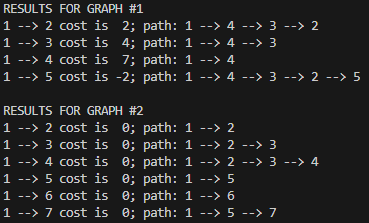
\includegraphics[width=0.8\textwidth]{./imgs/graphResult.PNG}}
    \caption{SSSP Terminal Output}
    \label{fig:figure2.16}
\end{figure}

\noindent
As is evident, each output lines up perfectly, no matter if the total weight ends up being positive or negative. The path also prints from the source Vertex to the current destination Vertex. Also, even though it looks weird, the reason why all of the weights in Graph \#2 are 0 is because all edges have a weight of 0. 

\subsection{Asymptotic Running Time of SSSP}

\noindent
It is important to note the time complexity of the Bellman-Ford algorithm when working with the linked objects implementation of the Graph. I am only focusing on the time complexity of the actual algorithm, not its output. The time complexity of SSSP is $O(|V| * |E|)$, where $V$ represents the set of Vertices in the graph, and $E$ represents the set of edges in the graph. The $||$ represent the cardinality of the sets, so the time complexity of the algorithm is the number of vertices times the number of edges. This is mostly because of the relaxation process. Each edge in the graph ($|E|$) is relaxed $|V| - 1$ times, and ignoring constants, it results in $O(|V| * |E|)$. Technically, there is a section of the algorithm where it checks for negative cycles, which is $O(|E|)$ since it loops through all edges once. But, since this isn't a dominant term, the time complexity for the Bellman-Ford SSSP algorithm still results in $O(|V| * |E|) + O(|E|) = O(|V| * |E|)$.

\section{Greedy Algorithms}
\setcounter{figure}{0} % Reset figure counter

\subsection{File Parser and Keywords}
\noindent
The final part of this assignment I will explain is the Greedy Algorithm implementation. To do this, the program first creates Spice objects, and then using those, a Fractional Knapsack algorithm is ran with different capacities. This algorithm outputs the combination of spices that maximizes the total value loaded into the knapsack. Before I explain the parsing I created for the spice.txt file, I want to explain some variables I created to help with the process. Below are declarations of some variables that are used for the parser:

\begin{figure}[H]
  \centering
  \lstinputlisting[firstline=104, firstnumber=104, lastline=109]{main.cpp} 
  \caption{Variable Declarations (main.cpp)}
  \label{fig:figure3.1}
\end{figure}

\noindent
\begin{itemize}
    \item The "mySpices" vector contains many Spice objects, which will be created throughout the parser (Line 105). This is where they are all stored.
    \item The "sortSpices" boolean will decide whether or not to sort the mySpices vector (Line 106). This variable is only set the false in the beginning, and once the first knapsack is created, the boolean will be set to true, and it will remain true for the rest of the program's duration, meaning this vector only gets sorted once.
    \item The "Index" integers are used to avoid putting magic numbers all over my program (Line 107). It is also important to note that this parser also uses the commandIndex constant declared earlier. Like in Section 2, each line of the file is put into a vector. These values are used to access certain indices of the vector.
\end{itemize}

\noindent
I had to read the file and understand all the keywords that were being used in order to create a parser and do tokenization based on each line in the file. Below is how I created a parser for the Spice file.

\begin{figure}[H]
  \centering
\lstinputlisting[firstline=111, firstnumber=111, lastline=164]{main.cpp} 
  \label{fig:figure3.2-part1}
\end{figure}

\begin{figure}[H]
  \centering
  \lstinputlisting[firstline=165, firstnumber=165, lastline=187]{main.cpp} 
  \caption{File Parsing for Fractional Knapsack Problem (main.cpp)}
  \label{fig:figure3.2-part2}
\end{figure}

\noindent
Like with the Dynamic Programming section, I first read all the words on a line and stored them in a vector. Then, I accessed the vector to process the data.

\vspace{1em}
\noindent
The first thing I needed to do was to read the file and store it in the file variable, which was declared earlier (Lines 112-117). After reading the entire file, I needed to process each line of the file (Line 120). There are a couple more local variables to help with the parsing process, like the stream variable (Line 122), the word string (Line 123), and the words vector (Line 124), which have all been explained in the previous section. They function the exact same as before.

\vspace{1em}
\noindent
However, there are a couple new local variables that are used for the Spice object, which are:
\begin{itemize}
    \item (Line 127) newSpice, which points to the newest created Spice object.
    \item (Line 128) name, which is a string that is the name of this Spice object.
    \item (Line 129) price, which is a float that is the total price of this Spice object.
    \item (Line 130) qty, which is an integer that is the quantity of this Spice object.
\end{itemize}

\noindent
Like before, the first section of the parser after the variable declarations is filling up the words vector with each word in the line. Each word in the line is read using the stream and word variables (Line 133). Depending on the word, the program will do the following:
\begin{itemize}
    \item If the word was a comment or was just empty, then no vector needs to be created and the loop is finished (Lines 136-138).
    \item If the word wasn't a comment, that means it is valuable information the program needs to know. Therefore, no matter what, the word will be added to the vector. However, exactly like before, there is a slight problem. Some of these words have semicolons at the back, which is no good when I have to deal with those values. If the word ends in a semicolon, it will be removed (Lines 142-145). Then, the word will be added to the words vector (Line 148).
\end{itemize}

\noindent
As is evident, the code I wrote is file specific, meaning it needs to be written in a certain way so the parser can work as intended. If the file format is different in any way, it won't work.

\vspace{1em}
\noindent
After each word in the line was written into the words vector, I needed to find out the possible options for each command. The two words that the commands can start with are "spice" or "knapsack", and I would have to ignore anything else. After checking if the vector actually had words in it (Line 151), I would need to check each word in order to fulfill its purpose.

\begin{itemize}
    \item If the word at the first index (Index 0) in the vector was "spice", that means that a new Spice would need be created (Line 154). If this is the case, it gets the name, total price, and quantity of the Spice (Lines 157-159). Because these values are all on the same line, they are all in the words vector, so the constant indices are used to retrieve these values. Using these values, a new Spice is created (Line 162) and it is added to the mySpices vector (Lines 163).
    \item If the word at the first index (Index 0) was "knapsack", that means the greedy algorithm needs to be ran. Firstly, if this was the first instance of the knapsack command being in the file, that means the mySpices vector needs to be sorted (Lines 168-172). 
    \begin{itemize}
        \item The Spices are sorted in descending order by its unit price value. The unit price is calculated in the constructor of the Spice class, which will be explained in Section 3.2. That means the Spice with the highest unit price will be in the first index of the vector, and the Spice with the lowest unit price will be in the last index of the vector. Like explained in the Introduction Section, the Sort file is very similar to how it was in previous Assignments, except I had to change it to make it sort unit prices, and also I had to make it sort in descending order, which was all very easy.
    \end{itemize}
    \item After the vector is sorted, the greedy algorithm is performed by calling the fKnapsack function (Line 175). This function also handles the output, so there is nothing to worry about for that in the parser. 
\end{itemize}

\noindent
After the parser finishes and the entire file is read, the Spices in the mySpices vector need to be deleted to avoid memory leaks. The program iterates through all the Spices in the vector and each Spice is deleted one by one (Lines 181-184). Then, the spice file is closed because all of the reading has finished (Line 186).

\vspace{1em}
\noindent
Like before, this implementation of the parser increased the readability and writability of my code. Debugging was easier because my code was easier to read, and writing out the program was easier once I understood the full process that I was trying to implement. 

\subsection{Spice Class}
\noindent
The Spice object and its members are extremely important when it comes to performing the Greedy Algorithm. Below is the implementation of the Spice class with its members: 

\begin{figure}[H]
  \centering
  \lstinputlisting[lastline=25]{Spice.h} 
  \caption{Spice Class (Spice.h)}
  \label{fig:figure3.3}
\end{figure}

\noindent
The members of the Vertex class are:
\begin{itemize}
    \item name, which is a string (Line 13), and stores the name of the Spice.
    \item price, which is a float (Line 14), and is the total price of the Spice depending on its quantity.
    \item qty, which is an integer (Line 15), and is the current quantity of the Spice.
    \item unitPrice, which is a float (Line 16), and is the unit price of just having one Spice. It may be easier to think of the unit price as the price of the Spice if the qty equals 1. It determines the price of each individual Spice.
\end{itemize}

\noindent
This class also has a parameterized constructor (Line 19), used when each Spice is created in the main parser. It sets each member of the object to the formal parameter passed in by the function (Line 21-23). It also calculates the unitPrice for this Spice, which is the total price divided by the quantity (Line 24).

\vspace{1em}
\noindent
This class also has getters to increase the readability of the program. Even though these members are technically private, and they can be accessed by any other file in the program, it looks cleaner when using getters, as shown below:

\begin{figure}[H]
  \centering
  \lstinputlisting[firstline=27, firstnumber=27]{Spice.h} 
  \caption{Spice Class Getters (Spice.h)}
  \label{fig:figure3.4}
\end{figure}

\noindent
All of these getters increase the readability of the code, especially in other functions when each member is needed, as shown on Lines 28 to 47.

\vspace{5em}

\subsection{Fractional Knapsack Algorithm}
\noindent
The goal of the fractional knapsack algorithm is to determine the combination of Spices that maximizes the total price value loaded into the knapsack. Depending on the capacity of the knapsack, and the unit price of each Spice, the maximum price output will be different. The function I'm about to explain is an example of a Greedy Algorithm. Greedy Algorithms always makes the choice that looks best at the moment. They make locally optimal choices and hope they lead to the globally optimal solution. This works for fractional knapsack problems, where items can be taken in fractions (like this), and it won't work for 0-1 knapsack problems, where items must be taken in whole. Below is my implementation of the fractional knapsack greedy algorithm:

\begin{figure}[H]
  \centering
  \lstinputlisting[firstline=26, firstnumber=26, lastline=59]{Greed.h} 
  \label{fig:figure3.5-part1}
\end{figure}

\begin{figure}[H]
  \centering
  \lstinputlisting[firstline=60, firstnumber=60, lastline=109]{Greed.h} 
  \caption{Fractional Knapsack Algorithm (Greed.h)}
  \label{fig:figure3.5-part2}
\end{figure}

\noindent
There are a lot of variables declared at the beginning of this function that need to be explained. These variables are very important for the functionality of the algorithm. These variables are:
\begin{itemize}
    \item (Line 30) curVal, which is an integer that counts the current iteration of the upcoming loop. This variable cannot surpass the value of the capacity, which is a formal parameter
    \item (Line 31) quantity, which is an integer that counts the current quantity for each Spice. Once this variable surpasses the qty member of the Spice, that means it is time to move on to the next Spice.
    \item (Line 33) curIndex, which is an integer that stores the current index of the Spice that is currently being worked on in the myItems vector (myItems is the same vector as the mySpices from main).
    \item (Line 34) quatloos, which is an integer that stores the total price of all Spices that made it in the knapsack. This is the result that will be printed in the output portion of this function.
    \item (Line 36) spiceSize, which is an integer that stores the size of the myItems (mySpices) vector.
    \item (Line 37) breakOut, which is a boolean that determines whether or not the upcoming loop should be broken out of early. This boolean is only set to true when there are no more Spices to iterate through (this can only happen if the capacity value is higher than the sum of all of the Spice's quantities).
    \item (Line 39) currentSpice, which points to the Spice that is currently being worked on. The first Spice that will be worked on is at index 0, which is shown on this line. Because this Spice is at the beginning of the myItems vector, that means that it has the highest unit price since it was sorted earlier in main.
    \item (Line 40) output, which is a vector of strings that stores the output for this function. This will be developed heavily later in this function.
    \item (Line 41) punctuation, which is a string that makes sure the punctuation of the output is correct.
\end{itemize}

\noindent
The function loops while the knapsack isn't at full capacity and if there are more Spices considered to be added to the knapsack (Line 44). A lot of things happen in this loop. First, the unit price of the current Spice is added to the quatloos value (Line 47) and the quantity integer is incremented since its unit price has been dealt with (Line 49). This quantity value is used to determine if the program should move on to the next Spice. 

\vspace{1em}
\noindent
If this value is equal to the current Spice's total quantity, that means the program needs to move on to the next Spice in the myItems vector (Line 52). For this, some output will be added to the output vector (Line 55) that displays the Spice's name and its quantity, the quantity count gets reset (Line 58), and it skips to the next Spice if there is one. If there is a Spice after the currentSpice, the currentSpice will become that Spice (Lines 62-65). If there isn't any Spice after the current Spice, the breakOut variable will be set to true and the loop will be broken out of (Line 66-70).

\vspace{1em}
\noindent
After that entire if statement was processed (the outer one involving the quantity values, not the inner one involving skipping to the next Spice), the curVal variable gets incremented (Line 73). This is to ensure that when the capacity is reached, it doesn't overflow the knapsack and the loop is cleanly exited. 

\vspace{1em}
\noindent
The greedy algorithm portion of the function has been completed at this point. The quatloos value is the maximum price that the knapsack can store given its capacity. The algorithm works mostly because the myItems vector was sorted in descending order by unit price. The rest of the function is purely for output and nice formatting.

\vspace{1em}
\noindent
If there was any more data to output from the loop, it gets added to the output vector (Lines 77-80). This case happens if the capacity value made the program exit the loop and there was still some Spice left over to process. The left over Spice does NOT get processed, but instead the current quantity of that Spice gets added to the output vector. After everything needed to output is in that vector, the results are finally printed to the terminal. The initial line of output is on Line 83, and then depending on the output vector, more output is printed. An edge case that is important to check is if the output vector is empty. If it is empty, that means nothing is in the knapsack (Lines 86-89), most likely because its capacity is 0. Then, all of the values from the output vector are printed using a loop (Line 92). For formatting, there is an extra if statement that determines whether or not the program is at the end of the line for output. If it is not at the end of the line, and there is still more output to come, it places a comma (Lines 95-98). However, if it is at the end of the line, it places a period (Lines 99-102). Then, the output from the vector is printed to the terminal (Line 105).

\vspace{1em}
\noindent
It could be helpful to think as the output vector as an array implementation of a Queue. It is essentially a Queue, where strings are enqueued, and when they need to be used, they are dequeued.

\vspace{1em}
\noindent
Below is example output for the fractional knapsack algorithm (unfortunately I cannot make it any larger, sorry, but digitally zooming in works perfectly fine):

\begin{figure}[H] 
    \centering 
    \fbox{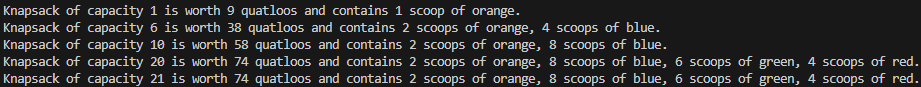
\includegraphics[width=0.98\textwidth]{./imgs/knapsackResult.PNG}}
    \caption{Fractional Knapsack Output}
    \label{fig:figure3.6}
\end{figure}

\vspace{1em}
\noindent
That was the entire fractional knapsack function, including its output portion. For me, it is difficult to start working on the function because I didn't know how I was going to output the results. However, once coming up with the idea of the output vector, it became a lot easier. After that, most of my time on the function was spent dealing with edge cases and special scenarios.


\subsection{Asymptotic Running Time of Fractional Knapsack}
\noindent
It is important to note the time complexity of the Fractional Knapsack when working with the Spice objects and the Greedy Algorithm. I am only focusing on the time complexity of the actual algorithm, not its output. The time complexity of Fractional Knapsack is technically $O(n * \log_2n)$, where $n$ represents the number of Spices that are being dealt with. This is because of the Quick sort algorithm, which needs to be used in order for this implementation to work. The reason that Quick sort has a running time of $O(n * \log_2n)$ is deeply explained in the Assignment 1 document. The complexity of the code inside of the fractional knapsack function is all dominated by this sorting function, so it doesn't matter what the complexity of that code is, because it is smaller than $O(n * \log_2n)$. But, in my opinion, this is kind of stupid, since it doesn't actually capture the complexity of the greedy algorithm. It just captures the complexity of a sort that was done before the greedy algorithm. So, with that being said, the time complexity of the fractional knapsack function, excluding the sorting algorithm, is $O(n)$, where $n$ represents the number of Spices that are being dealt with. This is because the loop for the function processes spices sequentially. In the worst case, it iterates through all spices, but only enough to fill the knapsack. An argument can be made where the time complexity is $O(n + c)$, where $c$ represents the capacity of the knapsack, since the loop when probably run more than once for each Spice. This value is independent of $n$ though, so it would be most likely be ignored when using asymptotic notation. Therefore, the function's time complexity is $O(n)$. This also proves that the overall time complexity is still $O(n * \log_2n)$, because $O(n * \log_2n)$ + $O(n)$ still equals $O(n * \log_2n)$. And, of course, ignoring the constant factor for the log, the ACTUAL time complexity for this ENTIRE section of the program would be $O(n * log\ n)$. 

\section{Conclusion}
\setcounter{figure}{0}
\begin{figure}[H] 
    \centering 
    \fbox{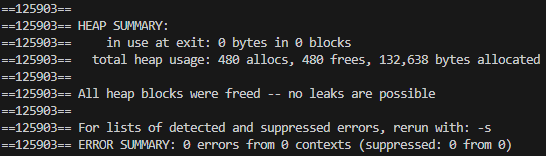
\includegraphics[width=0.98\textwidth]{./imgs/ValgrindOutput.PNG}}
    \caption{Valgrind Output (running command "valgrind ./main")}
    \label{fig:figure4.1}
\end{figure}

\noindent
Wow, again, this was a wild ride for me. AGAIN, I would like to apologize for this document being so long, but there was a lot of material to explain. This was an extremely great learning experience for me because I was touching upon areas that I've never touched on before. I've never implemented SSSP or a Greedy Algorithm before. Most of my time went into perfecting my implementations of these algorithms. I tried to make the format of my output perfect. Even though there were a lot of difficult parts of this assignment, there was a lot of code from Assignment 3 that I copied and pasted to this assignment, especially for the linked object implementation for the Graph. I still had to change a lot about it, but it eased my mind knowing that I've done some of this before. 

\vspace{1em}
\noindent
I used Valgrind a lot again to see if the unloading functions were working properly, and as shown in Figure 4.1, they are working perfectly since there are no memory leaks.

\vspace{1em}
\noindent
I actually had a great time working on all of these assignments. I learned a lot about C++ and a lot about programming in general. I tried improving my readability and writability in my programs throughout the course, and I tried my best the entire time. I hope you learned anything from any of the documents I've written. Thank you!

\end{document}
